\subsection{An\'alisis de tiempos en funci\'on de los parametros de entrada}
En esta seccion analizaremos de manera experimental como varían los tiempos de ejecución de los algoritmos descriptos, al variar el largo y el ancho de la matriz y la cantidad de sanguijuelas del sistema.
\subsubsection{Ancho en función del tiempo}
Para comenzar, tomaremos un parabrisas con 50 sanguijuelas, tal que estas solo toquen un punto de la discretización, y para una granularidad fija de $1.0$ iremos variando el largo del parabrisas. De esta manera, comenzaremos con un parabrisas de $50 \times 50$ luego uno de $60 \times 50$ y asi aumentando de manera lineal ambos parametros hasta llegar a un parabrisas de $100 \times 50$. Resolveremos cada uno de estos sistemas utilizando ambos metodos implementados (Gauss y Descomposición LU). Los resultados obtenidos pueden verse en el siguente grafico:

\begin{center}
 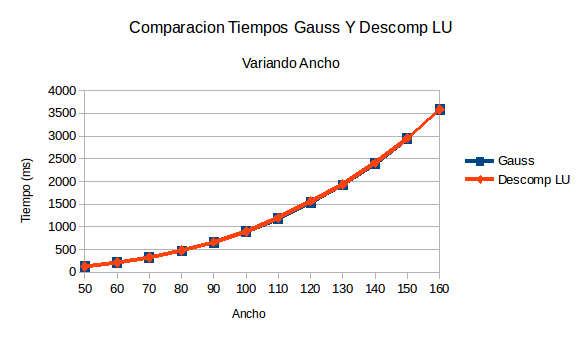
\includegraphics[width=400pt]{imagenes/testeo/anchoGauss.png}
\end{center}

Sabemos que al aumentar el largo de el parabrisas de manera lineal, aumentará de manera lineal el numero de ecuaciones en nuestra matriz de resolución. Lo que puede observarse en este grafico es que con un aumento lineal del largo del parabrisas, el tiempo de ejecución aumenta de manera cuasi-lineal. Esto era esperable ya que sabemos que tanto el gauss como la descomposición LU tienen una complejidad igual a $O(n*p^2)$, y dado que en nuestro modelado, utilizamos el largo del parabrisas para definir el tamaño de la banda en la matriz de resolución (osea $p$), era logico que al aumentar el largo, se obtuviera un aumento casi cuadratico en el tiempo de ejecución.
\\
Ademas en este grafico se pueden observar que tanto los tiempos de la factorización LU como la de gauss son similares.
\\
Ahora, utilizando la misma familia de parabrisas descripta anteriormente, veremos como se comportan ambos metodos de salvación. Dado que nos aseguramos que cada sanguijuela solo toque un punto de la discretización, nos aseguramos que podremos utilizar el metodo de Sherman Morrison. Para estos algoritmos, el grafico es el siguiente:
\\
\begin{center}
 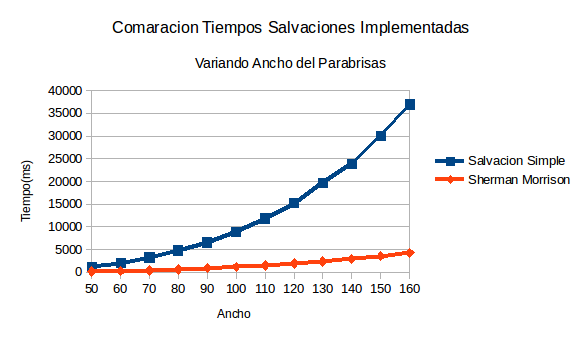
\includegraphics[width=400pt]{imagenes/testeo/anchoSalv.png}
\end{center}

Como era de esperar, el algoritmo que utiliza la optimización de Sherman morrison es mucho mas rapido y escala mejor que la versión simple que debe calcular todo el sistema desde cero, ademas el Sherman Morrison realiza operaciones sobre vectores y escalares haciendo la diferencia ahi en comparacion con el otro metodo.

\subsubsection{Largo en función del tiempo}
Ahora, analizaremos que sucede dejando fijo el ancho y variando el largo del parabrisas. Las condiciones son las mismas que en el test anterior, solo que ahora el ancho permaence constante igual a $50$ y se varía el largo de $50$ a $100$.

\begin{center}
 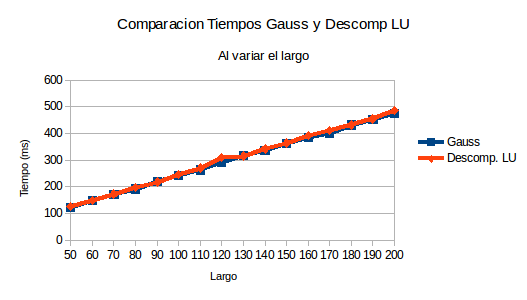
\includegraphics[width=400pt]{imagenes/testeo/largoGauss.png}
\end{center}

En este caso los tiempos de ejecución crecen de manera estrictamente lineal. Esto se debe que a diferencia del ancho, el largo no interviene en el calculo del tamaño de la banda de la matriz de resolución. Luego al aumentar el largo, solo aumenta la cantidad de incognitas $n$.
\\
Y aplicando el mismo experimento para los dos metodos de salvación:

\begin{center}
 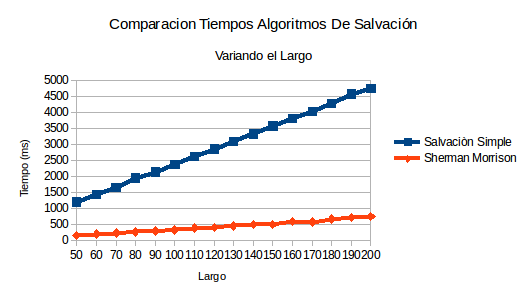
\includegraphics[width=400pt]{imagenes/testeo/largoSalv.png}
\end{center}

Al ignal que lo dicho en la seccion anterior, aqui tambien se puede ver las ventajas de utilizar sherman morrison. Ademas en este caso tambien puede apreciarse el comportamiento lineal del ambos algoritmos al variar el largo.

\subsubsection{Cantidad de sanguijuelas en función del tiempo}
Para el siguente experimento, variaremos la cantidad de sanguijuelas y dejaremos fija tanto la granularidad como el largo y el ancho del parabrisas. Nuevamente, por una cuestión de simplicidad las sanguijuelas solo tocarán un punto de la discretización. Para el experimento tomamos un parabrisas de $100 \times 100$, una granularidad igual a $1.0$, y variamos la cantidad de sanguijuelas desde $10$ hasta $100$. Resolviendo el sistema con el algoritmo de Gauss y Descomposicion LU, se obtuvo el siguiente grafico.

\begin{center}
 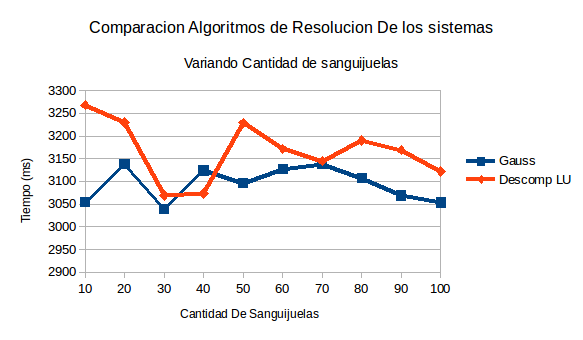
\includegraphics[width=400pt]{imagenes/testeo/sangGauss.png}
\end{center}

Como vemos, no se muestra ningun patron visible al modificar la cantidad de sanguijuelas del sistema. Esto es porque la cantidad de incognitas continua siendo la misma.
\\
Ahora utilizando el mismo experimento para el problema del ultimo disparo, resolviendo este parabrisas con ambos algoritmos, se obtuvo este grafico:

\begin{center}
 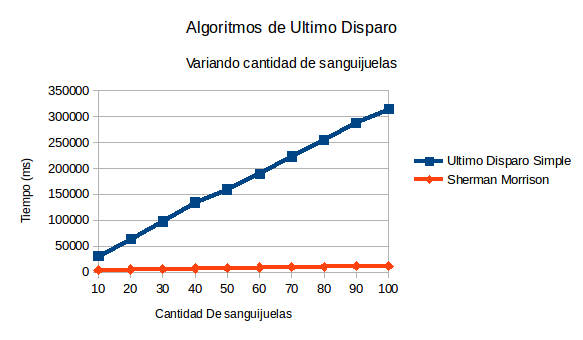
\includegraphics[width=400pt]{imagenes/testeo/sangSalv.png}
\end{center}

En este grafico se puede apreciar como si bien ambos algoritmos dependen de manera lineal de la cantidad de sanguijuelas, el algoritmo de sherman morrison presenta una mejor velocidad y una mejor escalabilidad.

\subsubsection{Granularidad en función del tiempo}
Por ultimo, veremos como afecta variar la granularidad de la discretización para ver como se ve afectada la performance. Para este experimento se dejarán fijos el largo y el ancho, iguales a $100$, la cantidad de sanguijuelas iguales a $5$ y se variará la granularidad desde $0.4$ hasta $0.9$, aumentando de $0.1$ en cada paso. Lo obtenido es lo siguiente:

\begin{center}
 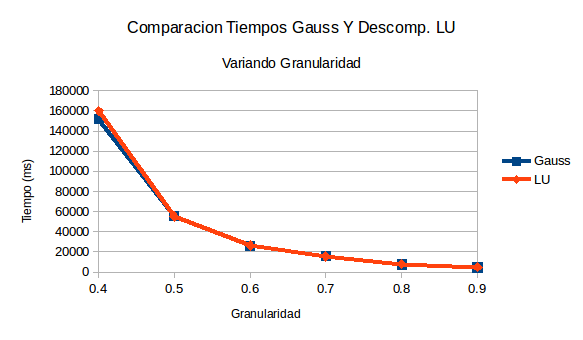
\includegraphics[width=400pt]{imagenes/testeo/granuGauss.png}
\end{center}

En el grafico puede verse que una disminucion lineal de la granularidad produce un aumento cuadratico en el tiempo de ejecución. Esto se debe a que tanto la cantidad de filas y la cantidad de columnas viene dado por el largo/ancho del paravrisas, dividido por la granularidad. Dado que el tamaño de nuestra matriz de resolución del probema viene dado por $\text{Cantidad De filas} \times \text{Cantidad De Columnas}$ esto será lo mismo que  $(\text{Largo} \times \text{Ancho}) / \text{granularidad}^2$. En esta formula puede verse claramente que disminuir la granularidad de manera lineal produce un aumento cuadratico en el numero de incognitas de nuestro problema.

\subsection{An\'alisis de temperatura funci\'on de las discretizaciones}
Partiendo de la base de que un aumento en la granularidad permite una mejor representaci\'on de las sanguijuelas (son circulos), notamos que con este aumento y mejora en la representaci\'on, el problema discreto parece al menos perceptualmente para el ojo humano, volverse continuo. Teniendo en cuenta esta informaci\'on, queda claro como una baja granularidad impacta directamente sobre la precisi\'on de los resultados (a expensas, como vimos con anterioridad, de los tiempos de c\'omputo).
\\
En el siguiente experimento, mostramos como varían los resultados al variar la granularidad:
\begin{itemize}
 \item Matriz $20 \times 20$, granularidad 2.\\
  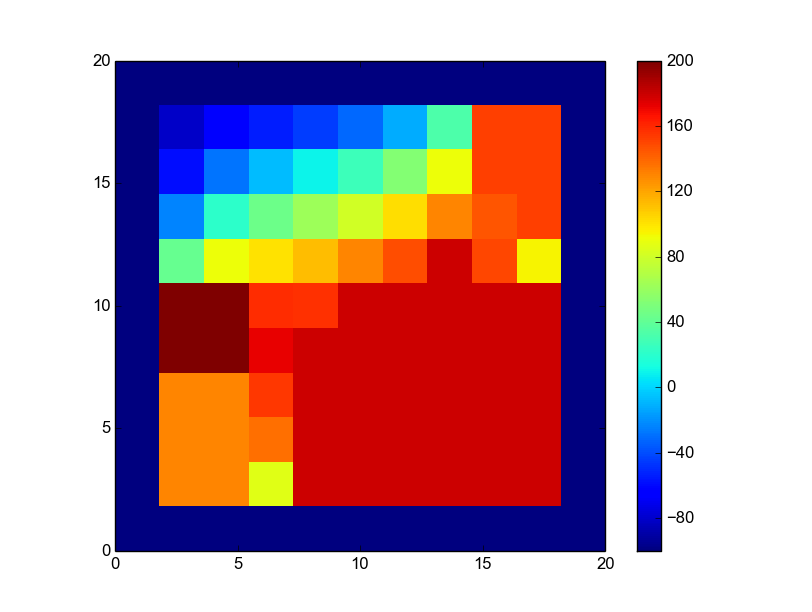
\includegraphics[width=400pt]{imagenes/imagen11.png}

 \item Matriz $20 \times 20$, granularidad 1.\\
  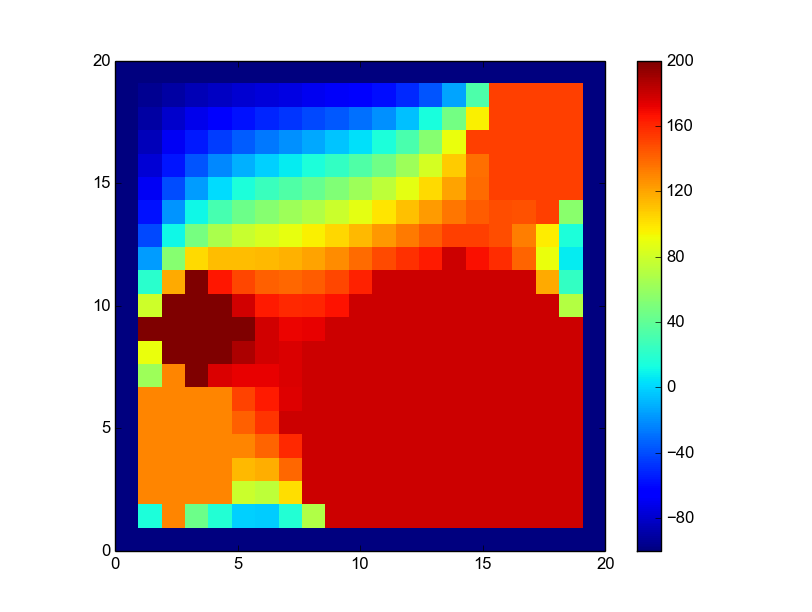
\includegraphics[width=400pt]{imagenes/imagen21.png}

 \item Matriz $20 \times 20$, granularidad 0,5.\\
  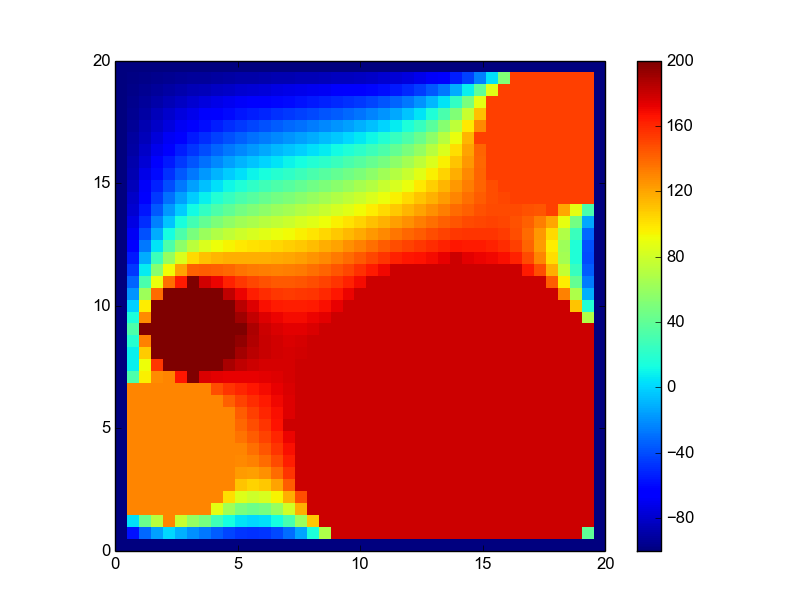
\includegraphics[width=400pt]{imagenes/imagen31.png}
  
   \item Matriz $20 \times 20$, granularidad 0,1.\\
  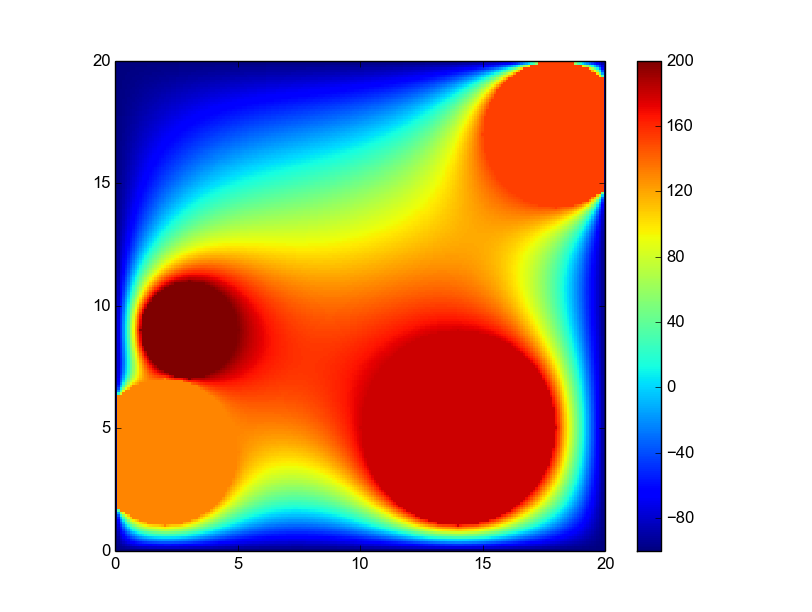
\includegraphics[width=400pt]{imagenes/imagen41.png}
\end{itemize}

Puede notarse a simple vista que una granularidad mas pequeña produce resultados que aproximan mas exactamente a lo que uno creería es el resultado real de la ecuación diferencial de la que partimos en la introducción ya que para una granularidad de $2$ pueden verse grandes bloques discretos, pero para la discretización de $0.1$ puede verse que estos bloques desaparecen y puede notarse una sierta 'suavidad' en el resultado obtenido, propio de una función continua y derivable, esto puede verse en el grafico ya que el la tonalidad va oscureciendo hasta llegar a rojo generando circulos grandes, de ser chicos estariamos viendo un pico en la funcion y no seria derivable.
\\
Ademas, a al disminuir la granularidad esta claro que la cantidad de incognitas cercanas al punto critico aumenta, por lo que, en caso de no poder tomarlo de manera exacta al menos podremos tomar un vecino muy proximo a este por lo que tenderíamos a pensar que la presición del resultado tambien aumentará por ese lado.
